\section*{Экспериментальные данные}

Зафиксируем показания термопары: $V_0 = 0.05$ мВ, $T_0 = 25\ {}^\circ$С. Снимем зависимость $f(V)$ и $f_0 (V)$, данные занесем в таблицу 1.
Погрешность измерения $V$ можно положить порядка $0.02$ мВ, $\sigma_f = 0.2$ кГц, $\sigma_{f_0} = 0.2$ кГц. Тогда $\sigma_T = 0.5\ {}^\circ$С. Погрешность $\varphi$:
\begin{equation*}
     \varphi = \frac{f^2}{f_0^2 - f^2},
     \hspace{10 mm} 
     \sigma_{\varphi(f, f_0)} = \left(2 \sigma_f + 2\frac{\sigma_f + \sigma_{f_0}}{f_0^2 - f^2}\right) \varphi(f, f_0),
\end{equation*}
данные также занесены в таблицу 1.

Построим зависимость $\sub{\varphi}{эксп}(T)$, зависимость отображена на графике 1.

\begin{figure}[h]
    \centering
    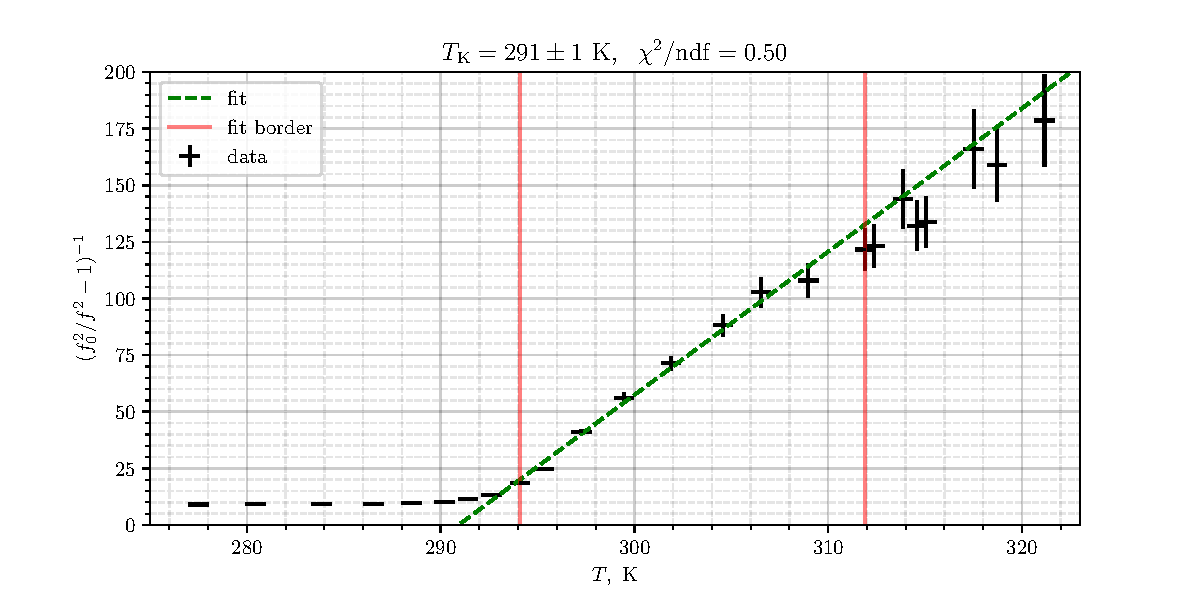
\includegraphics[width=0.9\textwidth]{plot.pdf}
    \caption{Лианеризуемая зависимость $\varphi(T)$}
    \label{fig:1}
\end{figure}


Зависимость $\sub{\varphi}{эксп}(T)$ аппроксимируем по МНК $\sub{f}{лин}(T) = a (T-\sub{T}{K})$, откуда находим
\begin{equation*}
    \sub{T}{K} = 291.5 \pm 1.0 \ \text{K},
\end{equation*}
что в пределах погрешности совпадает с табличным значением (292 К). Обменный интеграл тогда может быть найден, как
\begin{equation*}
    J = \frac{\sub{k}{b} \sub{T}{K}}{126} = \left(0.199 \pm 0.001\right)\ \text{мэВ}.
\end{equation*}


